\documentclass{article}

\usepackage[final]{neurips_2019}

\usepackage[utf8]{inputenc}
\usepackage[T1]{fontenc}
\usepackage{hyperref}
\usepackage{url}
\usepackage{booktabs}
\usepackage{amsfonts}
\usepackage{nicefrac}
\usepackage{microtype}
\usepackage{graphicx}
\usepackage{verbatim}
\usepackage{xcolor}
\usepackage{lipsum}
\usepackage{fullpage,enumitem,amsmath,amssymb,graphicx}
\newcommand{\note}[1]{\textcolor{blue}{{#1}}}
\hypersetup{colorlinks}
\title{
  Milestone Report: Translating Natural Language to Bash Commands using Deep Neural Networks \\
  \vspace{1em}
  \small{\normalfont Stanford CS224N Custom Project  }
}

\author{
 Daniel Jenson \\
  Department of Management Science \& Engineering \\
  Stanford University \\
  \texttt{djenson@stanford.edu} \\
  % Examples of more authors
  \And
  Yingxiao Liu \\
  Department of Civil and Environmental Engineering \\
  Stanford University \\
  \texttt{liuyx@stanford.edu} \\
  % Examples of more authors
%   \And
%   Name \\
%   Department of Computer Science \\
%   Stanford University \\
%   \texttt{name@stanford.edu} \\
%   \And
%   Name \\
%   Department of Computer Science \\
%   Stanford University \\
%   \texttt{name@stanford.edu}
}

\begin{document}

\maketitle

\begin{abstract}
	The objective of this project is to generate bash commands from natural
	language using a deep neural network. We are experimenting with several models,
	including GPT-2, BART, and T5, as well as different tokenization schemes to
	improve model performance on the NLC2CMD dataset. We have successfully
	trained a GPT-2 model, which has achieved modest performance. Next, we will
	next train models using BART and T-5. However, we suspect that the majority
	of gains may be achieved from improved encoding and tokenization.
\end{abstract}


\section{Key Information to include}
\begin{itemize}
	\item TA mentor: Ethan A. Chi
	\item External collaborators: No
	\item External mentor: No
	\item Sharing project: No
\end{itemize}

% {\color{red} This template does not contain the full instruction set for this assignment; please refer back to the milestone instructions PDF.}

\section{Approach}
The NLC2CMD Challenge was only held once at NeurIPS in 2020 and competing teams
put out working papers at best, but most often simply scattered notes across
Github. The dataset is simple a JSON consisting of translation pairs. Because
of this, a great deal of work had to go into preprocessing and encoding the
data, as well as becoming familiar with the HuggingFace infrastructure. We used
several trivial encodings to start, but found only one that achieves decent
performance, detailed in the dataset section. We found that the effectiveness
of the encoding varies by model and training objective, so this will have to be
tuned as we experiment with different models.
\par
The competition also provided several utilities of which we availed ourselves.
First, they released a bash to AST parser, which can also write an AST back to
a templated form, e.g. replacing file paths with ``File'' and regular
expressions with the token ``Regex.'' This allows the model to learn
placeholder values for commands. They also provided a function to compute their
competition scoring metric, which we use to establish our baseline.
\par
We used GPT-2 as our first base model, as most top competitors used this model
and it appears to provide a solid foundation for causal language modeling. We
also used the corresponding HuggingFace tokenizer. We experimented with BART,
but this model requires more work, as repurposing it for casual language
modeling has proven difficult; many original model weights are left
uninitialized, since this was not the original training objective of the model.
Our GPT-2 model achieved a performance of -0.20 using the evaluation criteria
provided by the competition, which is just shy of the -0.19 achieved by the
GPT-3 baseline.
\par

\section{Experiments}
\subsection{Dataset}
The dataset we used is from the ``The NLC2CMD Challenge'' hosted
\href{https://nlc2cmd.us-east.mybluemix.net/}{here}, consists of 10,000 parallel translations of English and bash. One example is like
\begin{verbatim}
ENG: Assign permissions 755 to directories in the current directory tree
CMD: find . -type d -print0 | xargs -0 chmod 755
\end{verbatim}
Since the bash examples consist specific directory paths, file names and permissions, we followed the guidance \href{https://github.com/IBM/clai/tree/nlc2cmd}{here} to parse the bash command into the corresponding template form as
\begin{verbatim}
CMD: find Path -type d -print0 | xargs -0 -I chmod Permission
\end{verbatim}
both to better capture the command structure and for simplicity. Finally, we grouped the English and the bash template together into the form
\begin{verbatim}
<eos_token> <ENG_token> <English> <CMD_token> <CMD_template> <eos_token> 
\end{verbatim}
by inserting tokens, which can be readily fed into the tokenizer provided by Huggingface. The dataset was then split into the training, validation and test sets with a ratio of 0.96 : 0.02 : 0.02.

\subsection{Evaluation method}
We used the cross entropy loss to train the model, but to measure the model performance, we used the metric similar to that defined by the competition, except only one prediction was sampled by the greedy algorithm (with a confidence of 1.0)
\begin{align*}
	S(p) & =\sum_{i\in[1,T]}\frac{1}{T}\times\left(
		\mathbb{I}[U(c)_i=U(C)i]\times\frac{1}{2}\left(
			1+\frac{1}{N}\left(X\right)\right) -\mathbb{I}[U(c)_i\ne U(C)_i]
		\right)                                                               
\end{align*}
where $U(x)$ is a sequence of bash utilities in a command $x$, $c$ is the predicted bash and $C$ is the ground truth bash. $X = 2\times |F(U(c)_i)\cap F(U(C)_i)| - |F(U(c)_i)\cup F(U(C)_i)|$ where $F(x)$ refers to the set of bash flags in a command $x$. $T$ is the maximum length between $U(c)$ and $U(C)$ while $N$ is the maximum size between $F(c)$ and $F(C)$. This is a very strict metric penalizing for both incorrect and unnecessary bash utilities/flags.
\subsection{Experimental Details}
We fine tuned a GPT-2 model from the Huggingface AutoModelForCausalLM pretrained models on our dataset. The number of epoch was chosen to be 5, since we found that although more epochs could help to reduce training loss, it harmed the evaluation performance of the model on the test set. The batch size was chosen to be 50, and an AdamW optimizer was used with an initial learning rate of 5e-5.

\subsection{Results}
The change of training loss during training has been plotted in the Figure 1 below. Initially, the loss decreased rapidly but after 3 epochs it became more or less stable at around 1.4. Further training can still reduce the loss, but the evaluation performance on the test set would be harmed.

\begin{figure}[ht!]
    \centering
    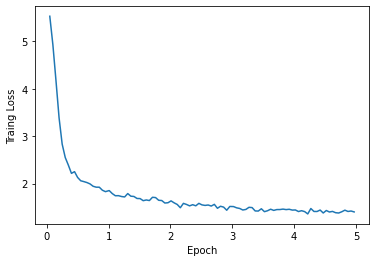
\includegraphics[width = 160px]{MilestoneReport/training_loss.png} 
    \caption{Change of training loss with number of epochs.}
    \label{overfitting}
\end{figure}

Using the evaluation metric defined previously, without any post processing of the prediction, the model can only achieve a score of -0.6 (a dummy model will get a score of -1.0 while an oracle will get 1.0). By doing an error analysis, we found that the model intended to output repeated sequences, or redundant pipelines, which were heavily penalized by the metric. Therefore, a post processing function has been added to remove adjacent repeated words, and limit the maximum number of pipelines to be 3. Then, our model can get a score of -0.21538. For comparison, the baseline model based on GPT-3 provided by the competition holder got a score of -0.19.

Also the score seemed to be far below 1.0, by taking a closer look at the model predictions, we can see the model actually did well. For most cases, the prediction is very close to or even exactly the same as the ground truth:
\begin{verbatim}
Prediction: find Path -nouser -exec rm {} \;
Truth     : find Path -nouser -ok rm {} \; 
\end{verbatim}
However, the model still tended to append wrong pipelines to the right predictions:
\begin{verbatim}
Prediction: cat File | sort -n -r | grep -v Regex
Truth     : cat File | sort -r -h 
\end{verbatim}
or even output repeated sequences:
\begin{verbatim}
Prediction: mount Regex -o remount,rw Regex mount Regex -o remount,rw 
            Regex mount Regex -o remount ...
Truth     : mount -o remount,ro -t yaffs2 Regex Regex 
\end{verbatim}
If the above errors can be fixed, the evaluation score will be significantly improved.


\section{Future work}
In future work, we will create a much larger dataset, as well as experiment
with different command line read-evaluate-print-loops (REPL). Outside of bash
AST parsing, this framework is REPL-agnostic and could be used for any
collection of structured commands. We will experiment with Nushell, a
recent shell written in Rust, which has much cleaner syntax than POSIX
compliant shells. Lastly, we will incorporate input selection for identifiers
to avoid using templated commands, similar to that used by Zhong, et
al\cite{zhong2017seq2sql}.


\bibliographystyle{unsrt}
\bibliography{references}

\end{document}
